\documentclass[12pt]{article}

\usepackage[utf8]{inputenc}
\usepackage[T1]{fontenc}
\usepackage[english]{babel}
\usepackage{tabularx}
\usepackage{hyperref}
\usepackage[margin=2cm,a4paper,headsep=1.2cm]{geometry}
\usepackage{ifthen}
\usepackage{fancyhdr}
\usepackage{tikz}
\usetikzlibrary{arrows}
\usetikzlibrary{arrows.meta}
\usepackage{graphicx}


\renewcommand{\baselinestretch}{1.1}
\setlength{\parindent}{0pt}
\setlength{\parskip}{1em}

\setlength{\headheight}{1cm}
\setlength{\headwidth}{\textwidth}

\makeatletter
\newcommand{\labeltext}[2]{%
  \@bsphack
  \csname phantomsection\endcsname % in case hyperref is used
  \def\@currentlabel{#1}{\label{#2}}%
  \@esphack
}
\makeatother    

\newcommand{\prio}[1]{\ifthenelse{\equal{#1}{1}}{low}{\ifthenelse{\equal{#1}{2}}{medium}{\ifthenelse{\equal{#1}{3}}{high}{\textbf{INVALID!}}}}\relax}

\newcounter{fr}
\newcommand{\fr}[8]{
\refstepcounter{fr}\label{#8}
\begin{tabularx}{16cm}{l|X}
 & \textbf{#1} \hfill \textbf{FR\arabic{fr}} \\ \hline
Description & #2\\ \hline
\ifthenelse{\equal{#3}{}}{}{Precondition & #3 \\ \hline}
\ifthenelse{\equal{#4}{}}{}{Postcondition & #4 \\ \hline}
Rationale & #5
\ifthenelse{\equal{#6}{}}{}{\\ \hline Dependencies & #6} 
\ifthenelse{\equal{#7}{}}{}{ \\ \hline Priority & \prio{#7}}
\end{tabularx}
\vspace*{0.75cm}
}

\newcommand{\actor}[4]{
\labeltext{#2}{#1}
\begin{tabularx}{16cm}{|l|X|}
\hline 
Actor: & #2 \\
\hline
Description: & #3 \\
\hline
Representative: & #4 \\
\hline
\end{tabularx}
}

%\newcommand{\rref}[1]{\ref{#1}\textsuperscript{$\rightarrow$ p. \pageref{#1}}}
\newcommand{\rref}[1]{\ref{#1}}
\newcommand{\frref}[1]{FR\ref{#1}\textsuperscript{$\rightarrow$ p. \pageref{#1}}}
\newcommand{\nfrref}[1]{QR\ref{#1}\textsuperscript{$\rightarrow$ p. \pageref{#1}}}

\newcommand{\myrule}[1]{
	\begin{tikzpicture}
		\draw[{Diamond[open]}-{Diamond[open]}, ultra thick] (0,0) to (#1, 0);
	\end{tikzpicture}
}

\renewcommand{\contentsname}{Table of Contents}

\begin{document}

% title page 
\begin{titlepage}

	\centering 
	\scshape 
	\vspace*{\baselineskip}
		
	\myrule{\linewidth}	
	\rule[1\baselineskip]{0.95\textwidth}{0.4pt}
    
    \Large
    User Manual
    \normalsize
   

	\rule[-1\baselineskip]{0.95\textwidth}{0.4pt}
	\myrule{\linewidth}
	
	\vspace{2\baselineskip}

    Flutter smart sensing library \\ for medical and psychological study apps
	
	
	\vspace*{15\baselineskip}
	
	edited by
	
	\vspace{0.55\baselineskip}
	
	{\scshape Leonhard Alkewitz, Florian Gebhardt, Hermann Fröhlich, \\ Mukhtar Muse, Felix Schlegel}
	
	\vspace{0.55\baselineskip}
	
	\vfill
	
\end{titlepage}


% table of contents
\tableofcontents
\thispagestyle{empty}

\newpage

% configure header and footer
\pagestyle{fancy}

\fancyhead[R]{\thepage}
\fancyhead[L]{\leftmark}
\fancyfoot{}

\section{Library}
\subsection{Installation}
\label{ssec:demoapp}
Installation instructions for the further development of the Smart Sensing Library:
\begin{itemize}
    \item Prerequisites:
        \begin{itemize}
        \item Make sure you have Flutter and Dart installed on your development machine.
        \item Check if you are using the latest version of the Flutter framework.
        \end{itemize}
    \item Clone the project:
        \begin{itemize}
        \item Open the command line or a suitable terminal on your computer.
        \item Navigate to the desired location for the project.
        \item Clone the project repository from version control (e.g. Git) using the following command:
\begin{verbatim}
git clone https://gitlab.uni-ulm.de/se-anwendungsprojekt-22-23
/smart-sensing-library.git
\end{verbatim}
        \end{itemize}
    \item Install dependencies
\footnote{
Note: Please ensure you have a stable internet connection to successfully download the dependencies during installation. 
Make sure all required SDKs and tools are up to date to ensure a smooth installation process.}:
        \begin{itemize}
        \item Navigate to the root directory of the Flutter project.
        \item Run the following command to install the required dependencies:
\begin{verbatim}
flutter pub get
\end{verbatim}
        \item Execute setup script
\begin{verbatim}
On Windows run:
powershell  .\setup.ps1

On Linux/macOS run:
bash bash setup.sh        
\end{verbatim}        
        \end{itemize}
    \item Configure emulator or device:
        \begin{itemize}
        \item Ensure that an emulator or physical device is properly configured.
        \item If using a physical device, connect your device via USB and enable developer mode.
        \end{itemize}
    \item Start the application:
        \begin{itemize}
        \item Open the command line or terminal and navigate to the \textit{example} directory of the Flutter project.
        \item Execute the following command to start the Flutter application:
\begin{verbatim}
 flutter run
\end{verbatim}        
        \end{itemize}
        

\end{itemize}

\subsection{Features}
The library is split into two core components: the Smart Sensing Library and the Sensing Plugin

The Smart Sensing Library contains most of the functions required by the customer. It serves as an access point for reading sensor data and was designed according to the principle of pipe-and-filter architecture. This gives the customer the ability to apply different filters to a data set and link them together. The library is divided into two main components: the IOManager and the API.

The API contains all the public methods that can be used by the customer to subscribe to sensors and retrieve filtered sensor data. The IOManager is responsible for managing all sensor data streams and writing them to the database. It also includes a buffer manager that speeds up access to the data. The Smart Sensing Library contains most of the functions required by the customer. It serves as an access point for reading sensor data and was designed according to the principle of pipe-and-filter architecture. This gives the customer the ability to apply different filters to a data set and link them together. 



\subsection{Api Methods}
We used Pigeon as our Api interface. Pigeon is a code generator tool that simplifies and makes more secure the communication between Flutter and the native platform.

Furthermore, you will now see a detailed explanation of the available API methods and how to use them. 
\begin{itemize}
    \item[\textbf{1.}] \texttt{isSensorAvailable(SensorId arg\_id): Future<bool>}
    
    This method checks if the specified sensor is available. It returns a boolean value indicating whether the sensor is available or not.
    
    \item[\textbf{2.}] \texttt{isSensorUsed(SensorId arg\_id): Future<bool>}
    
    This method checks if the specified sensor is currently in use. It returns a boolean value indicating whether the sensor is in use or not.

    \item[\textbf{3.}] \texttt{startSensorTracking(SensorId arg\_id, \\ int arg\_timeIntervalInMilliseconds): Future<ResultWrapper>}
    
    This method starts collecting sensor values for the specified sensor. It returns a ResultWrapper object indicating the status of the operation.

    \item[\textbf{4.}] \texttt{stopSensorTracking(SensorId arg\_id): Future<ResultWrapper>}
    
    This method stops collecting sensor values for the specified sensor. It returns a ResultWrapper object indicating the status of the operation.

    \item[\textbf{5.}] \texttt{changeSensorTimeInterval(SensorId arg\_sensorId, \\ int arg\_timeIntervalInMilliseconds): Future<ResultWrapper>}
    
    This method changes the acquisition interval for the specified sensor. It returns a ResultWrapper object indicating the status of the operation.

    \item[\textbf{6.}] \texttt{getSensorInfo(SensorId arg\_id): Future<InternalSensorInfo>}
    
    This method retrieves information about the specified sensor. It returns an InternalSensorInfo object that contains basic information about the sensor, such as the unit of sensor output data, accuracy, and supported sensor functions.
\end{itemize}

    You can use these methods to access sensor data and use it in your application.


\section{Demo App}

\subsection{Purpose}
    In addition, the library or the smart sensing plugin should be tested. This can be done by implementing a demo app using the library. In general, the demo app must be able to demonstrate the successful implementation of all functional requirements

\subsection{General Structure}
    The demo app follows a specific structure to provide a clear and organized user interface. It consists of various screens, navigation elements, and controls that allow developers to interactively explore the functionalities of the solution. The structure of the demo app facilitates navigation and access to the various features and options.

\subsection{Features of the demo app}
    The demo application offers a wide range of functions to facilitate the use and interaction with the sensors of your device. The various functions are explained in detail below: 
\begin{itemize}
    
    \item[1.]
    
    \begin{minipage}[t]{0.6\textwidth}
        The application is able to retrieve information on the smartphone and display it. This includes data such as model name, operating system version or free storage. If for some reason it is not possible to retrieve this information a notification or error message is displayed. This allows users to gain detailed insight into the technical aspects of their device. 
     \item[2.] They have the possibility to select a specific sensor and to track the measurements of this sensor. This allows users to monitor current sensor readings in real time. The application ensures that data from the selected sensor is continuously displayed.
    \item[3.] In addition to monitoring, the application provides the ability to customize the properties of a particular sensor. This includes changing the unit, time interval or precision for data acquisition. For example, you can change the sensor unit from $\frac{m}{s^2}$ to \textit{gal} or from \textit{kelvin} to \textit{celsius}. These adjustments allow users to customize the settings to their specific needs. 
    \end{minipage} 
    \hfill
     \begin{minipage}[t]{0.3\textwidth}
        \vspace{-\baselineskip}
        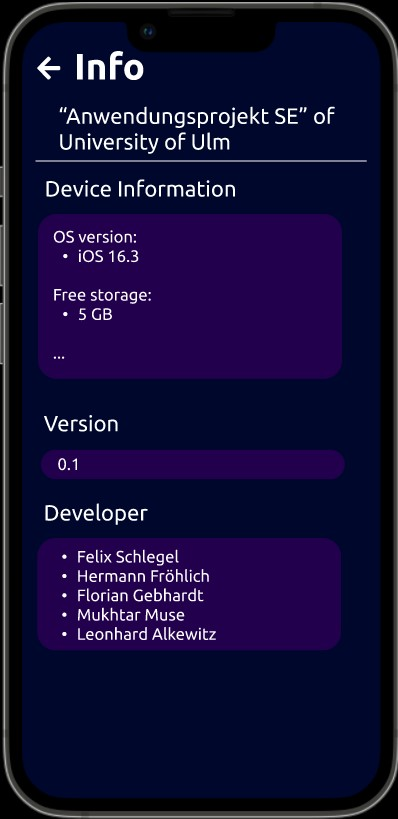
\includegraphics[width=\textwidth]{info.jpg}
    \end{minipage}
   

   \begin{minipage}[t]{0.3\textwidth}
    \vspace{-0.5\baselineskip}
    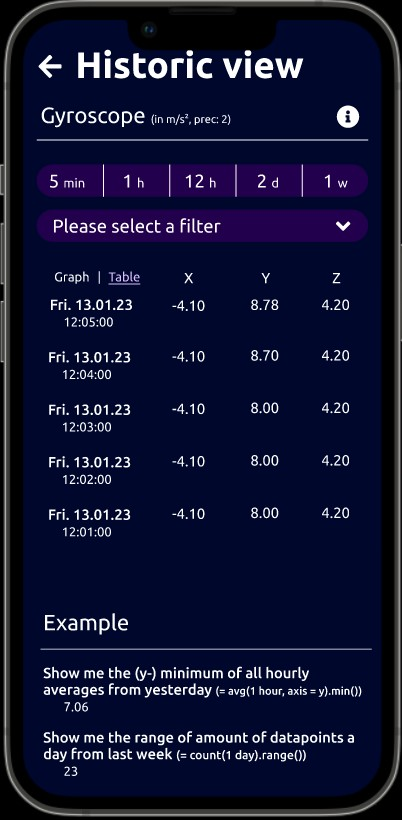
\includegraphics[width=\textwidth]{historic_view_page.jpg}
    \end{minipage} 
    \hfill
    \begin{minipage}[t]{0.6\textwidth}
    \item[4]
    If you want to stop tracking a specific sensor, you can select the corresponding option in the app. This will stop data collection for the sensor and update the readings display accordingly. Thus the users are able to only monitor sensors that are relevant to their current task.
    \item[5]
    The app also makes it easier to find a specific sensor. You can search for a sensor by entering its name or you can favorite the sensor and see it easier
    The search function helps users find the sensor they want from the list of available sensors on their device.This saves time and navigates through the different sensors.
    \item[6]
    By selecting a specific sensor in the app, users can view live data from that sensor. This allows them to monitor current readings in real life and see any changes or trends. For example, you can use to view current pressure and check current acceleration values. 
    \end{minipage}
    \item[7]
    In addition to viewing live data, users can also access processed or historical data from a specific sensor. This allows them to analyze and learn from previous and processed measurements. For example, they can view graphs based on the collected data or view previous measurements to identify trends or patterns.
\end{itemize}
    These advanced features provide application users with a complete way to interact with their application's sensors. They allow users to collect sensor data, adjust sensor parameters, and view them in real time.
    
\subsection{Usage of the library in the demo app}
    The demo app used the library extensively to collect, filter, and store sensor data. Here are the most important information about it:
    \begin{itemize}
        \item[1]Sensing Plugin as Submodule
        
        The Sensing Plugin, which is responsible for reading sensor data and pre-processing, was integrated into the demo app as a submodule. It establishes the connection to the iOS and Android devices and enables the reading of sensor data. For testing purposes, a FakeSensorManager was used to serve as a replacement for the actual SensorManager and simulate sensor data being read from the devices.
        \item[2] Implementation of the IO Manager
        The IO Manager was implemented as the main component to provide access to sensor data and manage its storage. The IO Manager integrates the appropriate filter tools and buffer manager to process and store sensor data. It serves as a central access point for all other components of the library.

        \item[3] Filter Tools and Buffer Manager

        The Filter Tools have been implemented to apply various filters to the sensor data. They allow the developer to manipulate the sensor data and extract specific values. The Buffer Manager is responsible for managing the sensor data streams and writing them to the database. It also contains a buffer memory to speed up access to the data.
        \item[4] The IO Manager as the main access point

        The IO Manager represents the main access point to obtain and store sensor data. All other components of the library, including the Sensing Plugin and Filter Tools, are used and managed by the IO Manager. This ensures consistent and efficient processing of sensor data.
      
        
  
    \end{itemize}
By using the library, specifically the Sensing Plugin, IO Manager and Filter Tools, the demo app was able to acquire, filter and store sensor data. This allowed the developer to create a robust and feature-rich application specific to the requirements.
\subsection{Demo App example}
\begin{verbatim}
    Future<SensorTaskResult> addSensor({
    required SensorId id,
    required SensorConfig config,
  }) async {
    SensorTaskResult result;
    try {
      if (_objectStore == null) {
        throw Exception("Database connection is not established. "
            "Establish connection first to use the IOManager.");
      }

      while (_sensorThreadLock) {
        await Future.delayed(Duration.zero);
      }

      if (_subscriptions[id] != null) {
        return SensorTaskResult.alreadyTrackingSensor;
      }

      _sensorThreadLock = true;

      result = await _sensorManager.startSensorTracking(
        id: id,
        config: config,
      );

      if (result == SensorTaskResult.success) {
        _bufferManager.addBuffer(id);
        _subscriptions[id] = _sensorManager.getSensorStream(id)!.listen(
              (sensorData) => _processSensorData(sensorData, id),
              onDone: () async => _onDataDone(id),
            );
      }
    } finally {
      _sensorThreadLock = false;
    }
    return result;
  }
\end{verbatim}
The ``addSensor`` method adds a sensor with the passed ``id``. The returned ``SensorTaskResult`` indicates whether the task was successful (``SensorTaskResult.success``) or not. Only if the task was successful, the sensor is subscribed and the data is collected.

The passed ``config`` is used to specify the sensor time interval and the properties of the sensor output data.If the database connection cannot be established It then throws an exception.
\subsection{Links}
For more information about the repository, documentation, etc.:


\textbf{Repository}
    \begin{itemize}
        \item \href{https://gitlab.uni-ulm.de/se-anwendungsprojekt-22-23/smart-sensing-library}{Smart Sensing Library}
        \item \href{https://gitlab.uni-ulm.de/se-anwendungsprojekt-22-23/sensing-plugin}{Sensing Plugin}
    \end{itemize}
 \textbf{Mockup}   
    \begin{itemize}
        \item \href{https://gitlab.uni-ulm.de/se-anwendungsprojekt-22-23/documentation/-/tree/master/Mockup}{Mockup}
    \end{itemize}
\textbf{Documentation}
\begin{itemize}
    \item \href{https://gitlab.uni-ulm.de/se-anwendungsprojekt-22-23/documentation/-/blob/master/Software%20design%20document/design_doc.pdf}{Software design document}
    \item \href{https://gitlab.uni-ulm.de/se-anwendungsprojekt-22-23/documentation/-/blob/master/Software%20requirements%20document/SRD.pdf}{Software requirements document}
\end{itemize}

    
 


\end{document}

% https://www.nuclino.com/articles/functional-requirements
%??
% https://savioglobal.com/blog/business-analysis/functional-requirements-document-frd-template-examples/ wirkt auch gut